\documentclass[12pt]{report}
\usepackage{geometry}
\usepackage{graphicx}
\usepackage{amsmath}
\usepackage{fancyhdr}
\usepackage{hyperref}
\usepackage{booktabs}    % For professional-looking tables
\usepackage{array}       % For extended column definitions
\usepackage{tabularx}    % For adjustable-width tables
\usepackage{longtable}

\geometry{margin=1in}
\hypersetup{
	colorlinks=true,  % Set to true to use colored text for links
	linkcolor=blue,   % Set the color for internal links (e.g., table of contents)
	urlcolor=blue,    % Set the color for external links
	citecolor=blue,   % Set the color for citations
	pdfborder={0 0 0} % Remove the border around links
}
\title{Aircraft Design 1 - Fall 2024 \\ Assignment }
\author{Smythe Cy Goforth Jr, Matthew Burnett \\ Group 6 \\ Instance: [first delivery]}
\date{Hours spent on assignment: [60]}

\begin{document}
	
	\maketitle
	\newpage

	\chapter{Introduction}
	
	The following report details the weight, balance, stability, and control of our aircraft design. The steps required to calculate the new specifications of our design are explored in detail throughout the following report. The first chapter of this report will explore the calculations and processes required to estimate the sizing of the aircraft tail using the V-bar method. Following this, in Chapter 3, the design's ultimate load factor will be calculated. In Chapter 4, the ultimate load factor will be used to determine the aircraft OEW and center of gravity using the Torenbeek handbook. Chapter 5 will then explore and propose the position of the center of gravity with respect to the fuselage (XLEMAC). Chapter 6 will then detail the aircraft scissor plot. Lastly, in Chapter 7, the final tail design will be compared to its initially calculated V-bar values.
	
	\chapter{Plain Tail Geometry}
	
	The V-Bar method will be used to size the horizontal and vertical tail planes in the following chapter. The tail planes are two diagonal planes angled together to form an inverted V-tail, both faces secured to one another and supported by a tail spar connecting to the wing.  
	
	\section{Coefficients of Volume}
	
	Since we are still early in the design stages of our aircraft, the V-bar method can be used to determine preliminary tail sizing. The formulas listed below are derived using statistical data on vertical and horizontal tail planes in similar aircraft, as well as allowing for the determination of the volume coefficients of the tailplanes. $V_h$ is our horizontal volume coefficient and $V_v$ is our vertical volume coefficient:
	
	\begin{align}
		V_h &= \frac{S_h \cdot l_h}{S \cdot c} \\
		V_v &= \frac{S_v \cdot l_v}{S \cdot b},
	\end{align}
	
	where:
	\begin{itemize}
		\item $S$: Wing area ($1550.005$ in\(^2\))
		\item $S_h$: Horizontal tail area ($54.25$ in\(^2\))
		\item $S_v$: Vertical tail area ($49.165$ in\(^2\))
		\item $l_h$: Horizontal tail arm ($40.316$ in)
		\item $l_v$: Vertical tail arm (same as $l_h$)
		\item $b$: Wingspan ($128.35$ in)
		\item $c$: Mean chord ($18$ in).
	\end{itemize}
	
	Using these inputs and the similarity of the Trinity Pro Drone, the coefficients calculated are:
	\begin{align}
		V_h &= 0.010994 \\
		V_v &= 0.009963.
	\end{align}
	
	\section{The Vertical Tail}
	
	The design of the vertical tail follows closely the Trinity Pro's vertical tail geometry due to the similarity in design requirements. The values used include:
	\begin{itemize}
		\item $S_v = 49.165$ in\(^2\)
		\item $l_v = 40.316$ in.
	\end{itemize}
	
	The quarter-chord sweep angle and taper ratio are both set to 0 due to the constraints of the inverted V-tail. The aspect ratio is set to 2.5. The mean aerodynamic chord (MAC) of the vertical tail is calculated to be $5.978$ in.
	
	\section{The Horizontal Tail}
	
	The horizontal tail design similarly uses Trinity Pro values:
	\begin{itemize}
		\item $S_h = 54.25$ in\(^2\)
		\item Aspect ratio = 2.5
		\item Thickness-to-chord ratio = 0.2.
	\end{itemize}
	
	The angle between the horizontal and vertical tail surfaces is determined to be $42.185^\circ$, ensuring the horizontal and vertical components match the required areas.
	
	\chapter{Load Factor}
	
	In this chapter, the generation of the V-n diagram is explored. The maximum load factor is calculated by considering both maneuver and gust loading, then applying a safety factor of 1.5. 
	
	\section{Maneuver Loading}
	
	The maneuver load factor is determined based on airworthiness certification requirements. Using the equation:
	\begin{align}
		n &= \frac{q \cdot C_{L_{\text{max}}}}{W/S},
	\end{align}
	where $q$ is the dynamic pressure, $C_{L_{\text{max}}}$ is the maximum lift coefficient, and $W/S$ is the wing loading. The stall speed corresponds to the intersection of $n=1$ on the V-n diagram.
	
	\begin{figure}[h!]
		\centering
		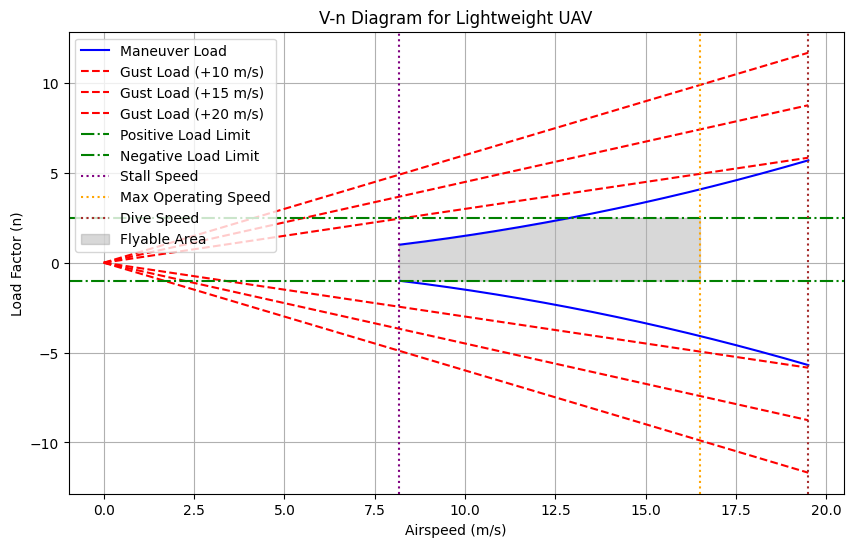
\includegraphics[width=6.5in]{Figures/VNdiagram.png} % Placeholder for technical drawings
		\caption{Maneuver loading diagram of the designed UAV}
		\label{fig:VNDIagram}
	\end{figure}
\newpage
\section{Chapter 4: Second Class Weight Estimation}

In the design process, minimizing aircraft weight is critical. Since most necessary component sizing has been completed for this aircraft, a more comprehensive second estimation of the aircraft weight needs to be completed in order to obtain a higher degree of accuracy. One issue, however, is that most second-class weight estimations are not intended for aircraft of our size or design regime. Thus, even though this weight estimation is likely to provide us with inaccurate results, it will be completed as if the aircraft were of the light aircraft or general aviation category. This will be done so that the aircraft designers may become more familiar with a critical aspect of aircraft design. In this chapter, the weight estimation will be completed using methods described and identified in the class II handbook. For our aircraft, we will employ the use of the Torenbeek method.

\subsection{Torenbeek Method}

The Torenbeek method uses a system of estimations grouped into 9 different weight groups for light aircraft whose averages are listed below. However, several of the groups are not included in our calculations as they cover aspects of aircraft that are not present in our design. These absent groups include the Engine Nacelle Group, the Surface Flight Controls group, and the Airframe Services group. The engine nacelle and surface flight control groups are not included in our second-class weight estimation as both of these features are not present within our design and thus do not need estimations. The Airframe Services group is not included as, for one, the majority of its weight contents are either similarly not present within the designed aircraft or are calculated using equations that are simply not scalable. In their place, the previously calculated weights of our control systems will be used to calculate control weight percentages instead of using the calculation provided by Torenbeek.

\begin{table}[h!]
	\centering
	\begin{tabular}{|l|l|}
		\hline
		\textbf{Weight Group} & \textbf{\%Wto} \\ \hline
		Airframe Structure & 14.2 \% \\ \hline
		Wing Weight & 2.73 \% \\ \hline
		Tail Group Weight & 11.1 \% \\ \hline
		Fuselage Body Group & 7.07 \% \\ \hline
		Landing Gear Group & 2.07 \% \\ \hline
		Propulsion Group & 1.60 \% \\ \hline
	\end{tabular}
	\caption{Weight groups for light aircraft (Torenbeek Method)}
\end{table}

Using the positive ultimate load \(N_{\text{ult}}\) of 3.75 calculated previously, with this value we can calculate the weight prediction of each group using the maximum takeoff weight calculated in Assignment 2 of 31.6 kg. In the following sections, the process behind the calculations of each of these groupings will be summarized.

\subsection{Airframe Structure}

The airframe structure weight can be calculated using the following equation:

\[
W_s = k_s \cdot W_{\text{to}} \cdot \left( \frac{b_f \cdot h_f \cdot l_f}{l_f} \right) \cdot N_{\text{ult}}
\]

Where:

\[
W_s = \text{Total airframe structure weight}, \quad W_{\text{to}} = \text{Take-off weight}, \quad k_s = \text{structure constant}
\]

Substituting the values:

\[
W_s = 0.447 \cdot 31.6 \, \text{kg} \cdot \left( \frac{0.2159 \cdot 0.19685 \cdot 0.82931}{0.82931} \right) \cdot 3.75
\]

\[
W_s = 5.58936 \, \text{kg}
\]

\subsection{Wing Weight}

The wing weight can be calculated using the equation:

\[
W_g = k_w \cdot \frac{b_s \cdot b_{\text{ref}} \cdot t_r}{S} \cdot N_{\text{ult}} \cdot f_{\text{ne}}
\]

Where:
\[
W_g = \text{Wing weight}, \quad k_w = \text{wing constant}, 
\]
\[
b_s = \text{Structural span}, \quad b_{\text{ref}} = \text{Reference span}, 
\]
\[
t_r = \text{Root chord thickness}
\]

Substituting the values:

\[
W_g = 31.6 \cdot \frac{3.74 \, \text{m} \cdot 1.905 \, \text{m} \cdot 0.25 \, \text{m}}{3.5 \, \text{m}^2} \cdot 3.75 \cdot 0.95
\]

\[
W_g = 1.52758 \, \text{kg}
\]

\subsection{Tail Weight Grouping}

The tail weight grouping can be calculated using the equation:

\[
W_{\text{tail}} = k_{\text{wt}} \cdot S_{\text{tail}} \cdot N_{\text{ult}}
\]

Where:

\[
W_{\text{tail}} = \text{Total tail weight}, \quad k_{\text{wt}} = \text{tail weight constant}, \quad S_{\text{tail}} = \text{Tail surface area}
\]

Substituting the values:

\[
W_{\text{tail}} = 0.64 \cdot 0.0667 \, \text{m}^2 \cdot 3.75
\]

\[
W_{\text{tail}} = 0.940275 \, \text{kg}
\]

\subsection{Fuselage Body Weight}

The weight of the fuselage body group is calculated as follows:

\[
W_f = k_{wf} \cdot V_d \cdot b_f \cdot h_f \cdot l_t \cdot S_g \cdot \Lambda \cdot N_{\text{ult}}
\]

Where:

\[
W_f = \text{Fuselage weight}, \quad k_{wf} = \text{Fuselage constant}, 
\]
\[
V_d = \text{Dive speed}, \quad S_g = \text{Gross Shell area}, 
\]
\[
\Lambda = \text{Fuselage fineness}
\]


Substituting the values:

\[
W_f = 0.23 \cdot 13.1226 \, \text{m/s} \cdot 0.2159 \, \text{m} \cdot 0.19685 \, \text{m} \cdot 1.024 \, \text{m} \cdot 0.503544 \, \text{m}^2 \cdot 4.24 \cdot 3.75
\]

\[
W_f = 21.6804 \, \text{kg}
\]

\subsection{Landing Gear Weight}

The landing gear weight group can be calculated with the following equation. Since we have three landing gears (two main and one on the nose), the calculation is run for each independent gear and then added together and totaled.

\[
W_{\text{uc}} = k_{\text{uc}} \cdot A_{\text{main}} \cdot W_{\text{to}} + B_{\text{main}} \cdot C_{\text{main}} + A_{\text{nose}} \cdot W_{\text{nose}} + C_{\text{nose}} \cdot W_{\text{to}}
\]

Where:

\[
W_{\text{uc}} = \text{Undercarriage weight}, \quad k_{\text{uc}} = \text{Constant for high wing},
\]
\[
A_{\text{main}}, B_{\text{main}}, C_{\text{main}} = \text{Coefficients for main gear},
\]
\[
A_{\text{nose}}, C_{\text{nose}} = \text{Coefficients for nose gear}
\]


Substituting the values:

\[
W_{\text{main}} = 22.2797 \, \text{kg}, \quad W_{\text{nose}} = 12.2859 \, \text{kg}
\]

\[
W_{\text{total}} = 56.8453 \, \text{kg}
\]

\subsection{Propulsion Weight Group}

The propulsion group can be calculated using the following equation:

\[
W_{\text{pg}} = k_{\text{pg}} \cdot N_e \cdot P_{\text{to}} + W_b
\]

Where:

\[
W_{\text{pg}} = \text{Propulsion weight}, \quad k_{\text{pg}} = \text{Propulsion constant}, 
\]
\[
P_{\text{to}} = \text{Takeoff power}, \quad W_b = \text{Battery weight}
\]


Substituting the values:

\[
W_{\text{pg}} = 1.16 \cdot 1 \cdot 4.54 \, \text{hp} + 8 \, \text{kg}
\]

\[
W_{\text{pg}} = 8.711807 \, \text{kg}
\]
\newpage
\subsection{Summary of Weight Groups}

The following table summarizes the weight groups calculated using the Torenbeek method.

\begin{table}[h!]
	\centering
	\begin{tabular}{|l|l|l|}
		\hline
		\textbf{Components} & \textbf{Weight [kg]} & \textbf{\%Wto} \\ \hline
		Aircraft Structure Weight & 5.58936 & 17.6 \\ \hline
		Wing Weight & 1.52758 & 4.8 \\ \hline
		Tail Weight & 0.940275 & 2.9 \\ \hline
		Fuselage Weight & 21.6804 & 68.6 \\ \hline
		Landing Gear Weight & 56.8453 & 178.89 \\ \hline
		Propulsion Weight & 8.711807 & 27.5 \\ \hline
	\end{tabular}
	\caption{Weight groups summary (Torenbeek Method)}
\end{table}

	\chapter{Center of Gravity Estimation}
	
	The center of gravity (COG) is calculated by dividing the aircraft into weight groups:
	\begin{itemize}
		\item Fuselage group
		\item Engine group
		\item Tail group
		\item Wing group
		\item Battery group(s)
		\item Payload group
	\end{itemize}
	
	Using the CAD model in conjunction with typical densities for the materials associated with each group, approximate weights of each major group were calculated. The OEW from the third order calculation was 24.8 Kg. Below are the weights of each group in addition to a plot displaying a middle wing configuration and the CG. 
	
	\begin{itemize}
		\item Fuselage group	7.03 Kg
		\item Engine group		1.04 Kg
		\item Tail group		2.99 Kg
		\item Wing group		5.44 Kg
		\item Battery group 1	4.13 Kg
		\item Battery group 2	4.13 Kg
		\item Payload group		0-7  Kg
	\end{itemize}
	
	\begin{figure}[h!]
		\centering
		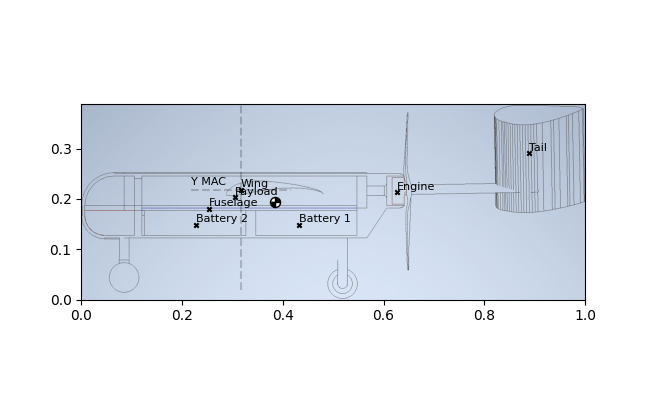
\includegraphics[width=6.5in]{Figures/CG_Calculation.png} % Placeholder for technical drawings
		\caption{Center of gravity by group and net center of gravity}
		\label{fig:CGPlot}
	\end{figure}

The plot below illustrates the relationship between the center of gravity as a fraction of the mean aerodynamic chord and the payload weight for different wing positions. The curves show how the aircraft's stability is affected as the payload weight increases. The shaded regions highlight the stability categories: the green region represents the stable range, while the orange and red regions indicate various levels of instability. The wing position was optimized to ensure that the center of gravity stays within the ideal stability range. This range is between 0.2 and 0.35 of the mean aerodynamic chord, where the aircraft maintains balance. Moving the center of gravity outside this range leads to increased instability, with the most extreme instability occurring when the center of gravity falls below 0.1 or exceeds 0.35. The plot helps visualize the impact of payload on the aircraft's stability across different wing positions.

	
	\begin{figure}[h!]
		\centering
		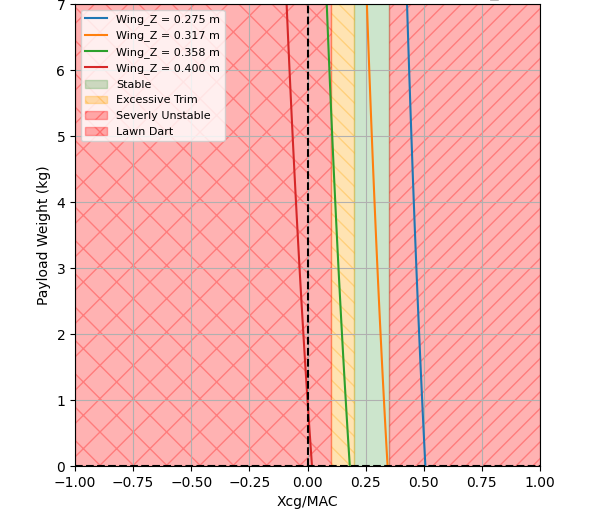
\includegraphics[width=6in]{Figures/Xcg_MAC_vs_Payload.png}
		\caption{Xcg/MAC vs Payload Weight for Various Wing Positions}
		\label{fig:Xcg_MAC}
	\end{figure}
	
\chapter{The Scissor Plot}

\section{Stability Curve}

The stability curve is derived from the following equation:

\begin{align}
	\frac{S_h}{S} = \frac{\bar{x}_{cg} - \bar{x}_{ac} + SM}{\frac{C_{L_{\alpha h}}}{C_{L_{\alpha}}} \cdot \left( 1 - \frac{d\epsilon}{d\alpha} \right) \cdot \frac{l_h}{c} \cdot \left( \frac{V_h}{V} \right)^2}.
\end{align}

Where:
\begin{itemize}
	\item \( \bar{x}_{cg} \) is the center of gravity location (fraction of MAC),
	\item \( \bar{x}_{ac} = 0.3 \) is the wing aerodynamic center (fraction of MAC),
	\item \( SM = 0.05 \) is the safety margin,
	\item \( C_{L_{\alpha h}} = 4.703 \, \text{rad}^{-1} \) is the tail lift curve slope,
	\item \( C_{L_{\alpha}} = 8.344 \, \text{rad}^{-1} \) is the aircraft lift curve slope,
	\item \( \frac{d\epsilon}{d\alpha} = 0.85 \) is the downwash factor,
	\item \( l_h = 5.0 \) is the tail arm to MAC ratio,
	\item \( V_h / V = 0.85 \) is the velocity ratio.
\end{itemize}

\begin{figure}[h!]
	\centering
	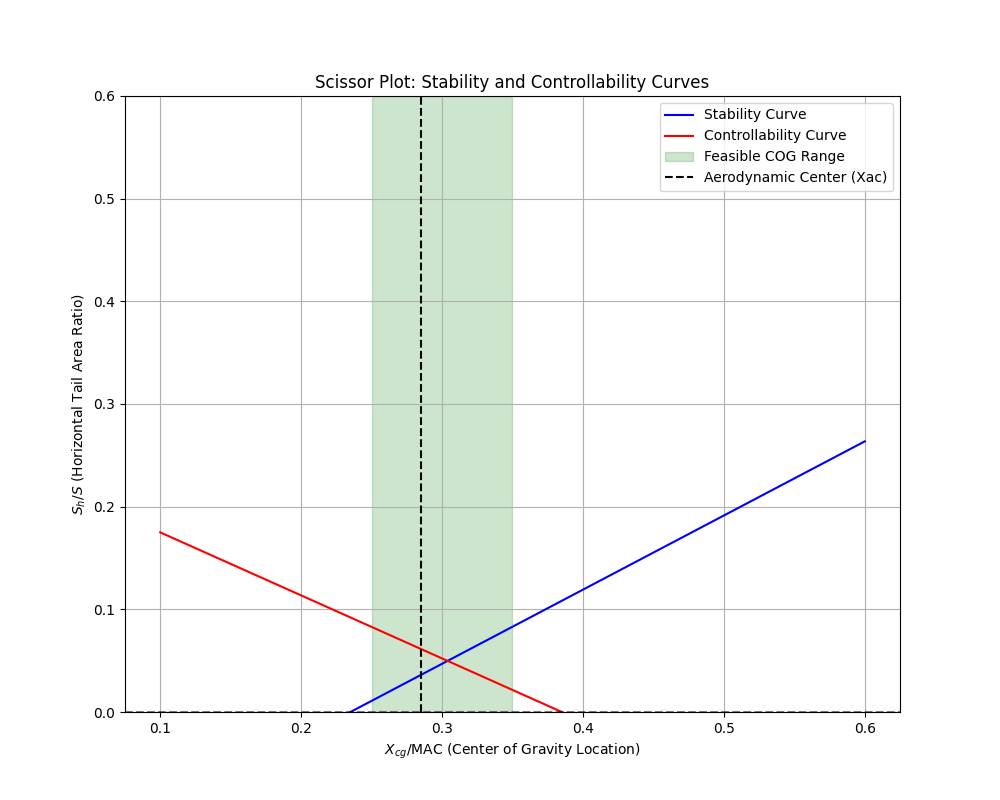
\includegraphics[width=5in]{Figures/Scissor_Plot.png}
	\caption{Stability Curve at the Maximum and Minimum Designed CG for the Selected Wing Position}
	\label{fig:StabilityPlot}
\end{figure}

\newpage

\section{Controllability Curve}

The controllability curve is given by:

\begin{align}
	\frac{S_h}{S} = \frac{C_{m_{ac}}}{C_{L_{\alpha}}} + \frac{\bar{x}_{cg} - \bar{x}_{ac}}{\frac{C_{L_{\alpha h}}}{C_{L_{\alpha}}} \cdot \frac{l_h}{c} \cdot \left( \frac{V_h}{V} \right)^2}.
\end{align}

Where:
\begin{itemize}
	\item \( C_{m_{ac}} = -0.15 \) is the moment coefficient at the aerodynamic center,
	\item \( \bar{x}_{cg} \) is the center of gravity location (fraction of MAC),
	\item \( \bar{x}_{ac} = 0.3 \) is the aerodynamic center (fraction of MAC),
	\item \( C_{L_{\alpha h}} = 4.703 \, \text{rad}^{-1} \) is the tail lift curve slope,
	\item \( C_{L_{\alpha}} = 8.344 \, \text{rad}^{-1} \) is the aircraft lift curve slope,
	\item \( l_h = 5.0 \) is the tail arm to MAC ratio,
	\item \( V_h / V = 0.85 \) is the velocity ratio.
\end{itemize}

The intersection of these two curves provides the minimum tail size and corresponding center of gravity location, where:

\[
\frac{S_h}{S} = 0.265 \quad \text{and} \quad \frac{X_{cg}}{MAC} = 0.425
\]

The two overlapping curves are shown below in the scissor plot:

\begin{figure}[h!]
	\centering
	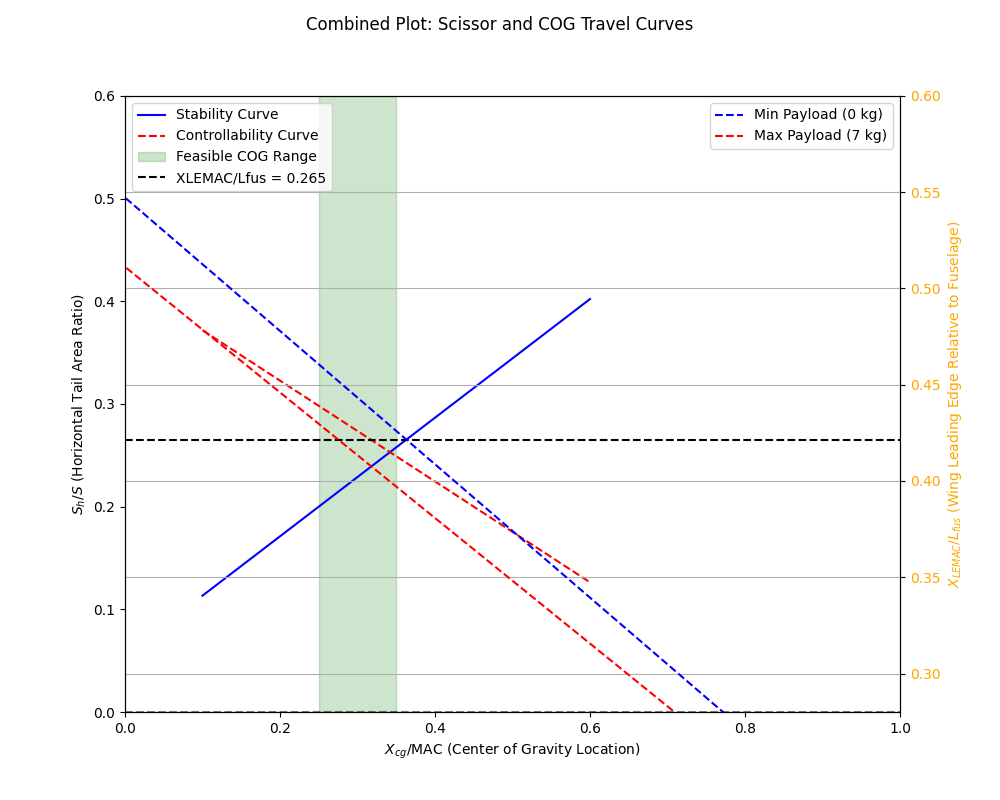
\includegraphics[width=6.5in]{Figures/Combined_Plot.png}
	\caption{Scissor Plot for Selected Wing Position}
	\label{fig:ScissorPlot}
\end{figure}

\chapter{Evaluation and Conclusion}

The final design of the aircraft tail was evaluated against the initial estimates. The scissor plot validated the stability and controllability requirements, confirming that the calculated values of \( \frac{S_h}{S} = 0.265 \) and \( \frac{X_{cg}}{MAC} = 0.425 \) are optimal for the given design. These values ensure that the aircraft remains within stable and controllable flight conditions, as evidenced by the analysis of both the stability and controllability curves. The design meets the required criteria for effective control and stability across the expected operational envelope.

\chapter{Stability and Control Analysis}

\section{The Stability Curve}

The stability curve is a critical tool for evaluating the aerodynamic stability of an aircraft. It demonstrates the relationship between the center of gravity (CG) and the required horizontal tail area ratio to maintain stability under various loading conditions. Several aerodynamic factors, such as the aircraft's lift curve slope, tail lift curve slope, and downwash effect, are considered in the analysis. These parameters influence the aircraft's pitch stability by determining how the tail counteracts the pitching moments generated by the wing.

\section{Stick-Fixed Neutral Curve}
Since the aircraft is battery-powered, with a static payload and a fixed battery weight, the stick-fixed neutral curve remains constant throughout the flight. The battery weight does not change, and the payload is stationary, meaning there is no dynamic redistribution of weight or shifting of the center of gravity (CG) during flight. Consequently, the neutral point, which defines the location where the total pitching moment remains fixed. As the battery and payload weights are constant, the stick-fixed neutral curve, which plots the relationship between CG position and required horizontal tail area for stability, does not change. This simplifies the stability analysis, as there is no need to account for changing aerodynamic moments or weight distribution during flight, allowing for a more straightforward assessment of the aircraft's stability and control based on the fixed weight distribution.

\subsection{The Aircraft Lift Coefficient without the Tail}

The aircraft's lift coefficient without the tail is primarily determined by the wing's lift curve slope, which for this analysis is \( C_L^\alpha = 8.344 \, \text{rad}^{-1} \). This value represents how the lift changes with the angle of attack, which directly affects the aircraft's ability to generate lift. Without the tail, the aircraft's overall stability depends heavily on the lift distribution across the wing and its interaction with the fuselage.

\subsection{The Wing Downwash Gradient Effect}

The downwash gradient effect refers to the downward deflection of airflow caused by the generation of lift on the wing. For this analysis, the downwash factor is set to \( 0.85 \), indicating that 15\% of the wing's lift is lost due to the downward airflow affecting the horizontal tail. This effect alters the angle of attack of the horizontal tail and plays a significant role in determining the aircraft’s stability. It helps to assess how the downwash influences the tail's effectiveness in countering pitching moments.

\subsection{The Lift-Rate Coefficient of the Horizontal Tail}

The lift-rate coefficient of the horizontal tail is influenced by the tail’s aerodynamic characteristics, including its surface area and the downwash effect from the wing. In this case, the tail lift curve slope is \( C_{L \alpha h} = 4.703 \, \text{rad}^{-1} \), which quantifies the tail's response to changes in the angle of attack. A positive lift-rate coefficient of the horizontal tail indicates that it contributes to the aircraft's overall stability by stabilizing the pitch moments generated by the wing.

\subsection{The Aerodynamic Centre of the Aircraft Without the Tail}

The aerodynamic center is the point at which the total aerodynamic moment is constant with respect to changes in the angle of attack. Without the tail, the aerodynamic center is located at a fixed point on the wing, typically around 25\% of the mean aerodynamic chord (MAC). This point is crucial for assessing the aircraft’s stability because it defines the balance between the pitching moments of the wing and the tail. The center of gravity's position relative to the aerodynamic center significantly affects the aircraft's stability.

\section{Forward Control Limit}

The forward control limit defines the maximum forward position of the center of gravity (CG) where the aircraft can still be controlled. When the CG exceeds this limit, the aircraft may experience uncontrollable pitching moments due to insufficient pitching moment from the horizontal tail.

\subsection{The Zero Lift Pitching Moment Coefficient}

The zero-lift pitching moment coefficient is defined as \( C_m^\text{ac} = -0.15 \), which represents the moment about the aerodynamic center of the wing when there is no lift. This coefficient helps determine the neutral point of the aircraft and plays a key role in assessing the control characteristics of the aircraft. A negative zero-lift pitching moment implies a tendency for the aircraft to pitch nose-down when lift is zero.

\subsection{Controllability Curve}

The controllability curve illustrates the relationship between the center of gravity (CG) and the ability of the aircraft to remain controllable. It shows how the required horizontal tail area to maintain control changes with the CG. As the CG moves forward, the required tail area increases, but beyond a certain point, the aircraft becomes uncontrollable. This curve is essential for understanding the impact of CG position on the aircraft’s stability and control.

\section{The Scissor Plot}

The scissor plot is a graphical tool that helps evaluate the stability of an aircraft by showing the relationship between the center of gravity (CG) and the aerodynamic center. It is used to determine the stability margins, which indicate how far the CG is from the aerodynamic center. A larger stability margin indicates greater stability, while a smaller margin suggests reduced stability. The scissor plot helps identify the optimal configurations that ensure sufficient stability for the aircraft.

\chapter{Evaluation and Conclusion}

The stability analysis has provided valuable insights into the design and performance of the aircraft. By evaluating the lift coefficient without the tail, the downwash gradient effect, and the lift-rate coefficient of the horizontal tail, we gained a better understanding of how these factors contribute to the aircraft's overall stability. The forward control limit and zero-lift pitching moment coefficient were used to define the stability boundaries, while the controllability curve and scissor plot helped evaluate the aircraft's control characteristics. The analysis ensured that the aircraft remains stable and controllable under a range of loading conditions and flight configurations, confirming that the design meets the stability and control requirements for safe operation.


			\begin{thebibliography}{99}
				
				% T-Motor References
				\bibitem{tmotor_v10}
				T-Motor, "V10 VTOL Motor," \url{https://store.tmotor.com/product/v10-vtol-motor.html}.
				
				\bibitem{tmotor_v10l}
				T-Motor, "V10L VTOL Motor," \url{https://store.tmotor.com/product/v10l-vtol-motor.html}.
				
				\bibitem{tmotor_v13l}
				T-Motor, "V13L VTOL Motor," \url{https://store.tmotor.com/product/v13l-vtol-motor.html}.
								
				% General Information
				\bibitem{faa}
				Federal Aviation Administration, "14 CFR Part 48," \url{https://www.faa.gov/air_traffic/publications/atpubs/aim_html/chap11_section_2.html}.
				
				% Aircraft References
				\bibitem{applied_aeronautics}
				Applied Aeronautics, "Applied Aeronautics," \url{https://www.unmannedsystemstechnology.com/company/applied-aeronautics/}.
				
				\bibitem{uavos_sat_i}
				UAVOS, "SAT-i," \url{https://www.uavos.com/products/fixed-wing-uavs/sat-i/}.
				
				\bibitem{uavos_sitaria_e}
				UAVOS, "SITARIA E," \url{https://www.uavos.com/products/fixed-wing-uavs/sitaria-e/}.
				
				\bibitem{uavos_borey_10}
				UAVOS, "BOREY 10," \url{https://www.uavos.com/products/fixed-wing-uavs/borey-10/}.
				
				\bibitem{aeromapper}
				Aeromapper, "Aeromapper," \url{https://www.directindustry.com/prod/aeromapper/product-182310-1802491.html}.
				
				\bibitem{insitu_scaneagle}
				Insitu, "ScanEagle Product Card," \url{https://www.insitu.com/wp-content/uploads/2020/12/ScanEagle_ProductCard_DU120320.pdf}.
				
				\bibitem{eos}
				EOS Technology, "Strix 300," \url{https://www.eos-technologie.com/strix-300/}.
				
				\bibitem{c_astral}
				C-Astral, "Unmanned Aircraft Systems," \url{https://pdf.directindustry.com/pdf/c-astral/unamanned-aircraft-systems/182250-945853.html#open2113345}.
				
				\bibitem{quantum_systems}
				Quantum Systems, "Trinity PRO," \url{https://quantum-systems.com/trinity-pro/}.
				
				\bibitem{geo_matching_dt26x}
				Geo-Matching, "DT26X LiDAR," \url{https://geo-matching.com/products/dt26x-lidar}.
				
				\bibitem{direct_industry_delair}
				DirectIndustry, "Delair," \url{https://www.directindustry.com/prod/delair/product-108459-1800225.html}.
				
				\bibitem{geo_matching_bramor_sar}
				Geo-Matching, "C-Astral Bramor SAR," \url{https://geo-matching.com/products/c-astral-bramor-sar}.
				
				\bibitem{aeromao_vtnaut}
				Aeromao, "VTNAUT," \url{https://aeromao.com/products/vtnaut/}.
				
				\bibitem{aeroexpo}
				AeroExpo, "UAV Factory Ltd. Europe," \url{https://www.aeroexpo.online/prod/uav-factory-ltd-europe/product-174156-793.html}.
				
				\bibitem{griffon_outlaw}
				Griffon Aerospace, "Outlaw G2," \url{https://www.griffonaerospace.com/products/outlaw-g2/}.
				
				\bibitem{unmanned_systems_pd1}
				Unmanned Systems Technology, "PD-1 Fixed Wing UAV," \url{https://www.unmannedsystemstechnology.com/wp-content/uploads/2016/06/PD-1-Fixed-Wing-UAV.pdf}.
				
				\bibitem{c_astral_bramor_c4eye}
				C-Astral, "Bramor C4Eye," \url{https://www.c-astral.com/en/unmanned-systems/bramor-c4eye}.
				
				\bibitem{satuav}
				Satuav, "Glider Drone Runway Drone," \url{https://www.satuav.com/glider-drone-runway-drone/long-endurance-fixed-wing-drone.html}.
				
				\bibitem{uav_systems_talon_gt}
				UAV Systems International, "Talon GT Drone," \url{https://uavsystemsinternational.com/products/talon-gt-drone}.
				
				\bibitem{uav_systems_skywalker}
				UAV Systems International, "Skywalker Drone," \url{https://uavsystemsinternational.com/products/skywalker-drone}.
				
				\bibitem{ua_sp}
				UA SP, "Altavian," \url{https://www.ua-sp.com/altavian}.
				
				\bibitem{insitu_integrator}
				Insitu, "Integrator," \url{https://www.insitu.com/products/integrator}.
				    % USC PowerPoint Slides
				\bibitem{usc_prelim_sizing1}
				University of South Carolina, "Preliminary Sizing 1," AESP 415 Lecture Notes, Version 3, \url{https://www.example.com/AESP415_001_06-PreliminarySizing1_V3}.
				
				\bibitem{usc_prelim_sizing2}
				University of South Carolina, "Preliminary Sizing 2," AESP 415 Lecture Notes, Version 3, \url{https://www.example.com/AESP415_001_06-PreliminarySizing2_V3}.
				
				
				
							
			
		\end{thebibliography}
		
		\newpage
		
		\section*{Appendix A: Power and Propulsion Aircraft Parameters Table}
		\begin{table}[h!]
			\centering
				\caption{Current Aircraft Propulsion and Flight Parameters for the UAV }
			\begin{tabular}{|l|l|l|l|}
				\hline
				\textbf{Symbol}    & \textbf{Parameters}                  & \textbf{Value}    & \textbf{Unit} \\ \hline
				\multicolumn{4}{|l|}{\textbf{Wing Characteristics}}                                                        \\ \hline
				
				b                 & Wing span                             & 3.26              & m²            \\ \hline
				A                 & Aspect ratio                          & 3                 & \_             \\ \hline
				\multicolumn{4}{|l|}{\textbf{Weights and Loadings}}                                                          \\ \hline
				$W_{TO}$            & Maximum takeoff weight                & 31.6              & kg            \\ \hline
				$W_{OE}$            & Operational empty weight              & 25.0              & kg            \\ \hline
				$W_{Payload}$       & Payload weight                        & 6.60              & kg            \\ \hline
				$W_{Battery1}$      & Battery weight 					       & 8.00              & kg            \\ \hline
				W/S               & Wing loading                          & 100               & N/m²          \\ \hline
				P/W               & Power-to-weight ratio                 & 0.086             & kW/kg         \\ \hline
				\multicolumn{4}{|l|}{\textbf{Flight Parameters}}                                                           \\ \hline
				$V_{cruise}$        & Cruise speed                          & 15         & m/s           \\ \hline
				$h_{cruise}$        & Cruise altitude                       & 122               & m             \\ \hline
				Endurance         & Endurance                             & 3.15              & hours         \\ \hline
				Range             & Range                                 & 47.21             & km            \\ \hline
			\end{tabular}

		\end{table}
\end{document}